\documentclass[11pt,notes=hide,aspectratio=169,mathserif]{beamer}

% PACKAGES
\usepackage{graphics}  % Support for images/figures
\usepackage{graphicx}  % Includes the \resizebox command
\usepackage{tikz}      % For flowcharts
\usetikzlibrary{arrows.meta, positioning} % Libraries for TikZ


\usepackage{url}	   % Includes \urldef and \url commands
\usepackage{natbib}
\usepackage{bibentry}  % Includes the \nobibliography command
\usepackage{verbatim}  %Supports comments
\usepackage{booktabs} %Supports \toprule, \bottomrule, etc in tables
\usepackage{etoolbox}  %Supports toggle commands
\usepackage{datetime}
\usepackage{bm}	%Supports bold math \bm
%the LaTeX standard:
\usepackage{cmbright}
\setbeamerfont{frametitle}{family=\fontfamily{cmbr}\selectfont,size=\Large}
\fontencoding{OT1}\fontfamily{cmbr}\selectfont

% PACKAGES (that should already be included by your LyX document settings)
\usepackage{amsfonts}  % Lots of stuff, including \mathbb 
\usepackage{amsmath}   % Standard math package
\usepackage{amsthm}    % Includes the comment functions
\usepackage{subcaption}

% CUSTOM DEFINITIONS
\def\newblock{} %Get beamer to cooperate with BibTeX
\linespread{1.2}

% IDENTIFYING INFORMATION
\title[class]{ECON 326: Economics of Developing Countries \\ TA Session 8}
\author[vaidehi's class ]{Vaidehi Parameswaran (Northwestern Econ)}
\date{\monthname[\the\month] \the\year}

% THEMATIC OPTIONS
%\setbeamercovered{transparent}
\usetheme{metropolis}
\definecolor{mycolor}{RGB}{48,7,144} 
\setbeamercolor{frametitle}{bg=mycolor, fg=white} % Frame title color
\setbeamercolor{title separator}{fg=mycolor} 
\setbeamercolor{progress bar}{fg=mycolor} 
\beamertemplatenavigationsymbolsempty
\setbeamertemplate{footline}[frame number]{}
\setbeamertemplate{itemize item}{\small\raisebox{1pt}{\textcolor{mycolor}{$\blacktriangleright$}}}
\setbeamertemplate{itemize subitem}{\footnotesize\raisebox{1pt}{\textcolor{mycolor}{$\triangleright$}}}
\setbeamertemplate{itemize subsubitem}{\tiny\raisebox{1pt}{\textcolor{mycolor}{$\triangleright$}}}

% BACKUP SLIDE NUMBERING
\usepackage{appendixnumberbeamer}

\begin{document}

%---------------------------------------------------------------------
\begin{frame}[plain]
\titlepage
\end{frame}
%---------------------------------------------------------------------


%---------------------------------------------------------------------
\begin{frame}{Today's Agenda}

\begin{itemize}
\item \href{https://onlinelibrary-wiley-com.turing.library.northwestern.edu/doi/epdf/10.3982/ECTA18916}{\textcolor{blue}{Fujiwara (2015)}}
\item \href{https://academic.oup.com/restud/article/92/1/339/7627149}{\textcolor{blue}{Gulzar and Khan (2025)}}
\item \href{https://www.lse.ac.uk/economics/Assets/Documents/personal-pages/robin-burgess/the-brazilian-amazons-double-reversal-of-fortune-manuscript.pdf}{\textcolor{blue}{Burgess et al. (2019)}}
\item The Curse of Natural Resources
\end{itemize}
\end{frame}
%---------------------------------------------------------------------

%---------------------------------------------------------------------
\begin{frame}{What is political economy?}

\begin{itemize}
\item When traditional approaches in economics are not enough to explain economic development
\item What are some themes in political economy?
\begin{itemize}
    \item Context matters - where and when 
    \item Role of culture and institutions
    \item Role of the state
    \item Conflict and cooperation
\end{itemize}
\end{itemize}
\end{frame}
%---------------------------------------------------------------------

\section*{\href{https://onlinelibrary-wiley-com.turing.library.northwestern.edu/doi/epdf/10.3982/ECTA18916}{\textcolor{blue}{Fujiwara (2015)}} \\[5mm] 
\textnormal{\small{Voting Technology, Political Responsiveness, and Infant Health: Evidence from Brazil}}}

%---------------------------------------------------------------------
\begin{frame}{This Paper}

\begin{itemize}
\item Political process can affect public goods provision and redistribution
\item This paper provides evidence on how improved political participation of poorer voters can enable targeted policies 
\item Uses the introduction of the Electronic Voting Machine in Brazil 
\item Affects who gets elected, public health care spending, utilisation, infant health outcomes
\item Focus: the intensive margin - universal suffrage already exists
\end{itemize}
\end{frame}
%---------------------------------------------------------------------

%---------------------------------------------------------------------
\begin{frame}{Background}

\begin{itemize}
\item Electoral systems can de facto disenfranchise certain groups
\item In Brazil, filling a ballot was not so trivial 
\begin{itemize}
    \item 23\% of adults cannot read or write a simple note 
    \item Paper ballots required voters to write down their vote and read instructions
\end{itemize}
\item Substantial error-ridden and blank votes (\textit{residual votes}) as a result 
\item EV technology introduced in 1990s as a substitute for paper ballots
\item Reduced residual votes was a spillover effect
\end{itemize}
\end{frame}
%---------------------------------------------------------------------

%---------------------------------------------------------------------
\begin{frame}{Why does EV make voting easier?}

\begin{itemize}
\item Provides visual aids - photos of candidates
\item Guides the user through the several votes that need to be cast 
\item Machine provides feedback 
\item Number based interface 
\end{itemize}
\end{frame}
%---------------------------------------------------------------------

%---------------------------------------------------------------------
\begin{frame}{Pre-reform}
\begin{figure}
\centering
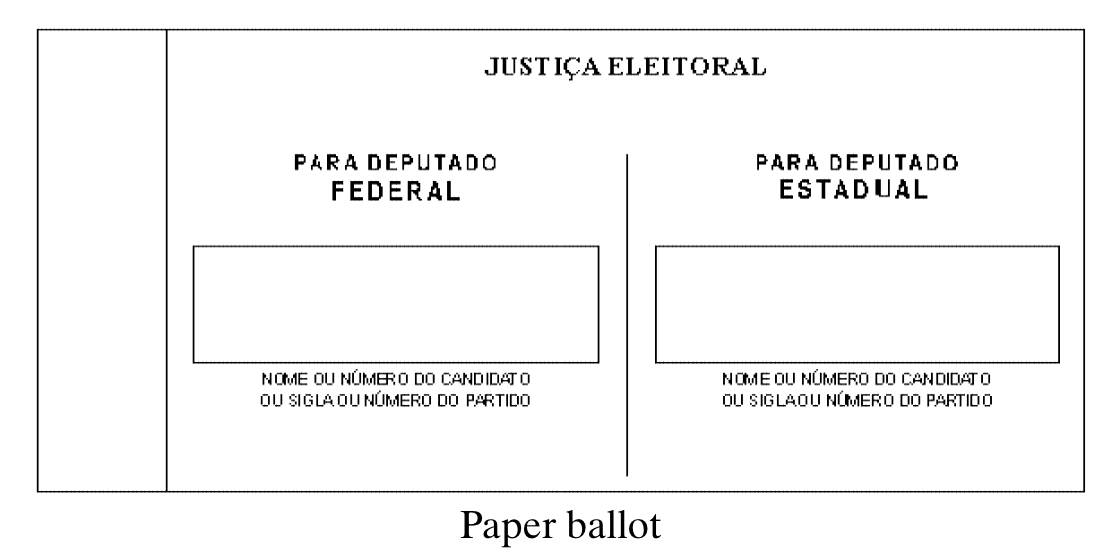
\includegraphics[width=0.8\textwidth]{inputs/fig1.png}
\end{figure}
\end{frame}
%---------------------------------------------------------------------

%---------------------------------------------------------------------
\begin{frame}{Post-reform}
\begin{figure}
\centering
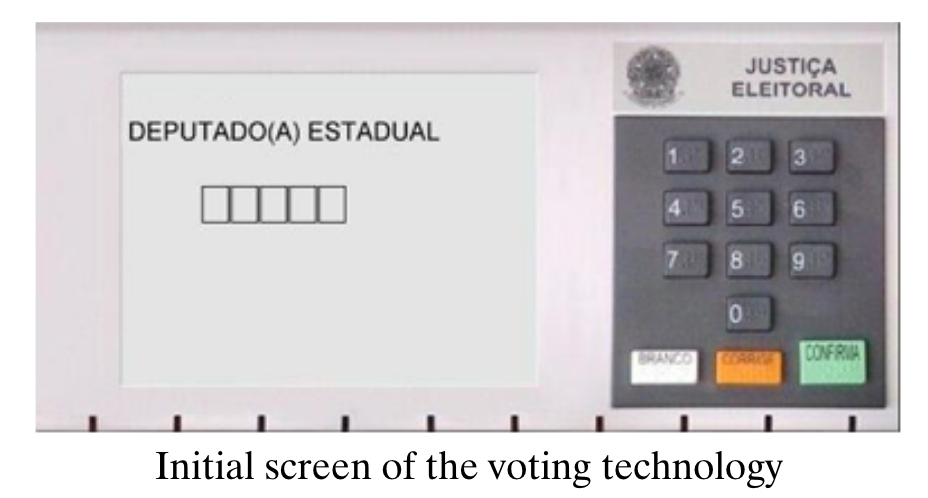
\includegraphics[width=0.8\textwidth]{inputs/fig2.png}
\end{figure}
\end{frame}
%---------------------------------------------------------------------

%---------------------------------------------------------------------
\begin{frame}{Post-reform}
\begin{figure}
\centering
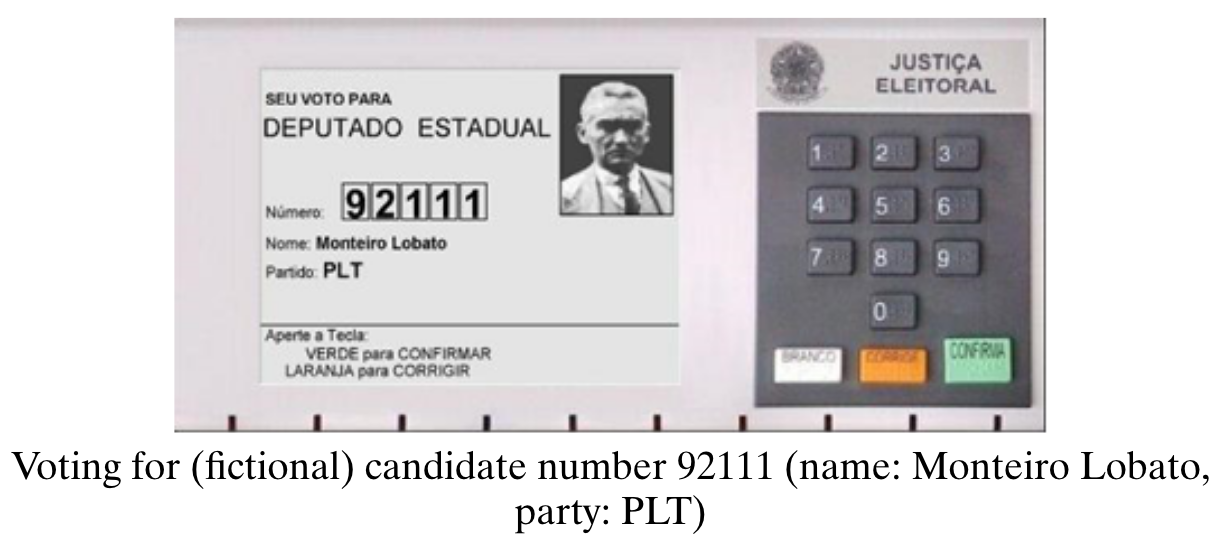
\includegraphics[width=0.8\textwidth]{inputs/fig3.png}
\end{figure}
\end{frame}
%---------------------------------------------------------------------

%---------------------------------------------------------------------
\begin{frame}{Post-reform}
\begin{figure}
\centering
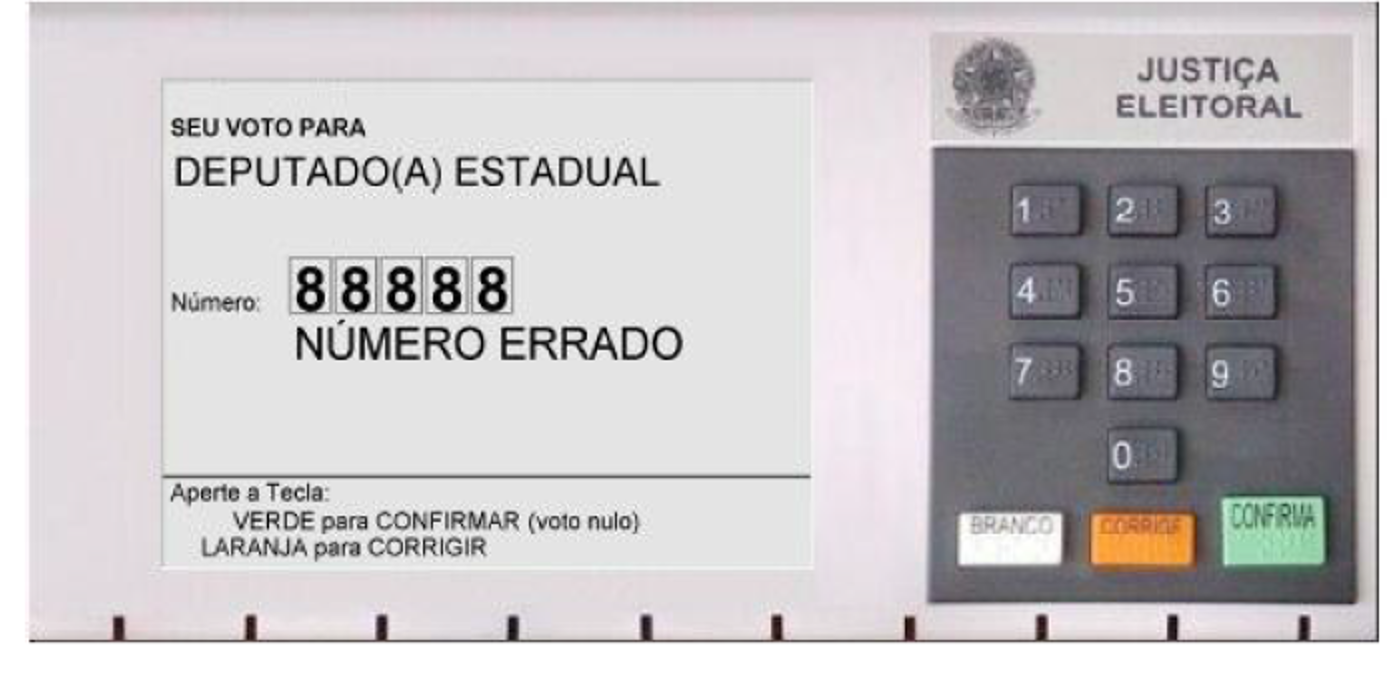
\includegraphics[width=0.8\textwidth]{inputs/fig4.png}
\end{figure}
\end{frame}
%---------------------------------------------------------------------

%---------------------------------------------------------------------
\begin{frame}{Empirical Strategy}

\begin{itemize}
\item In 1990 and 1994 elections, only paper ballots were used
\item In 1998 election, EV introduced 
\begin{itemize}
    \item Production capacity constraints 
    \item So only municipalities with $\geq$ 40,550 voters got EV 
    \item Threshold rule - naturally leads to ...?
\end{itemize}
\item In 2002, only EV used in all municipalities
\pause \item RDD in 1998 election: compare municipalities just above/below 40,500 voters
\pause \item Use 1994 and 2002 elections for placebo tests 
\end{itemize}
\end{frame}
%---------------------------------------------------------------------

%---------------------------------------------------------------------
\begin{frame}{Estimation Framework}

\begin{itemize}
\item $ TE = lim_{v_m \downarrow 40,500} E[y_m| v_m] - lim_{v_m \uparrow 40,500} E[y_m| v_m] $
\item Estimated effects are ``local'' - apply only to municipalities right around the threshold
\item The regression is equivalent to an OLS regression using only observations with $v_m \in [40,500 - h, 40,500 + h]$:
\begin{align*}
    y_m = \alpha + \beta 1\{v_m \geq 40,500\} + \gamma v_m + \delta v_m 1\{v_m \geq 40,500\} + \epsilon_m
\end{align*}
\item $\beta$ is the treatment effect
\end{itemize}
\end{frame}
%---------------------------------------------------------------------

%---------------------------------------------------------------------
\begin{frame}{RDD in Pictures}
\begin{figure}
\centering
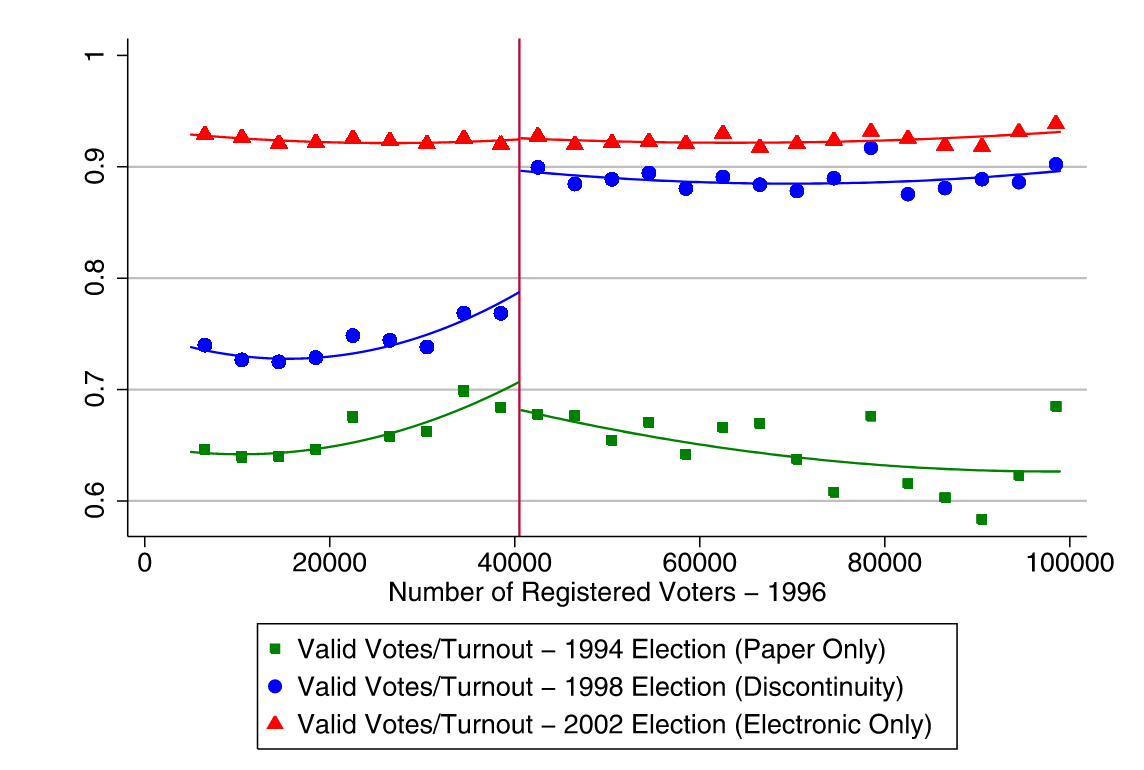
\includegraphics[width=0.55\textwidth]{inputs/fig5.png}
\end{figure}
\begin{itemize}
\pause \item Jump from 75\% to 95\% upon crossing the cutoff
\pause \item No such jumps in 1994 and 2002 - valid treatment and control groups
\pause \item Such large shares are probably erroneous votes, not just abstentions
\end{itemize}
\end{frame}
%---------------------------------------------------------------------

%---------------------------------------------------------------------
\begin{frame}{Who benefits?}
\begin{figure}
\centering
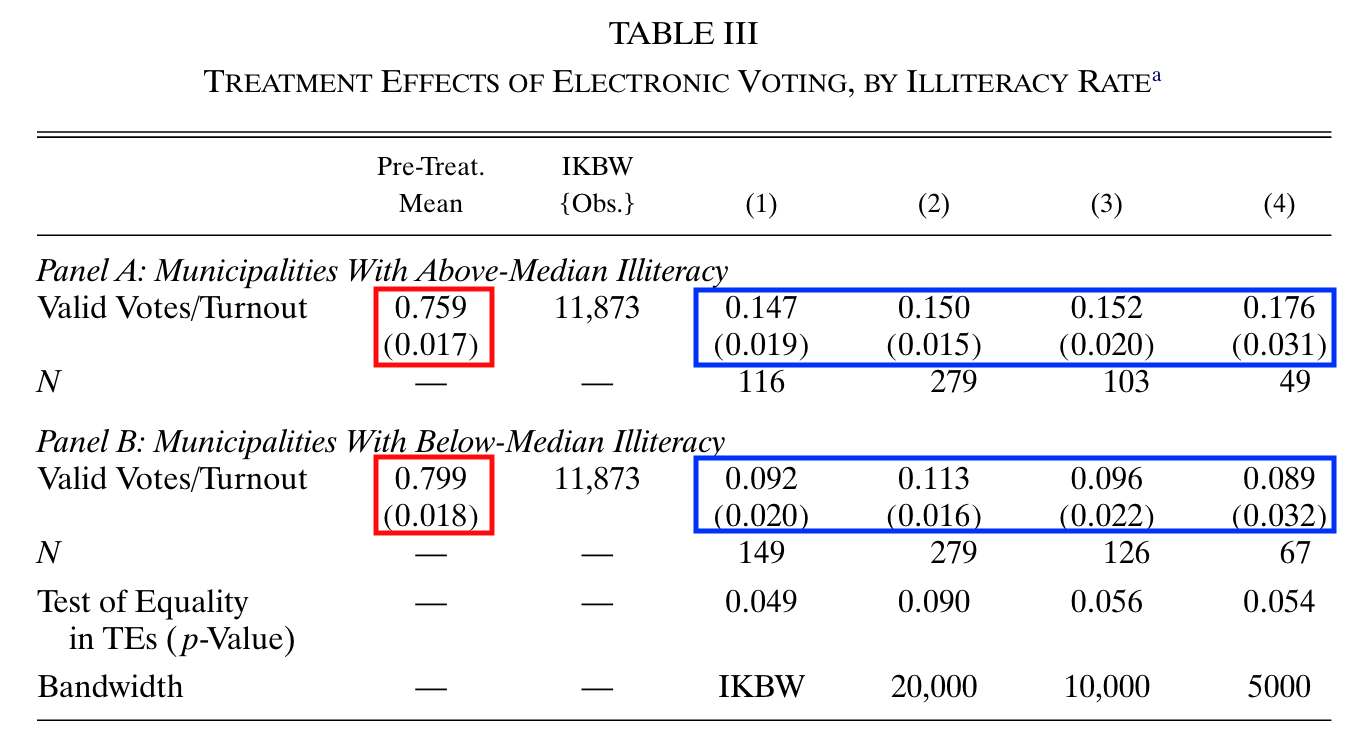
\includegraphics[width=0.7\textwidth]{inputs/fig6.png}
\end{figure}
\begin{itemize}
\pause \item Split sample based on illiteracy
\pause \item Consistent narrative that less educated people had more difficulty with paper ballots
\end{itemize}
\end{frame}
%---------------------------------------------------------------------

%---------------------------------------------------------------------
\begin{frame}{Political Participation and Policy}
\begin{figure}
\centering
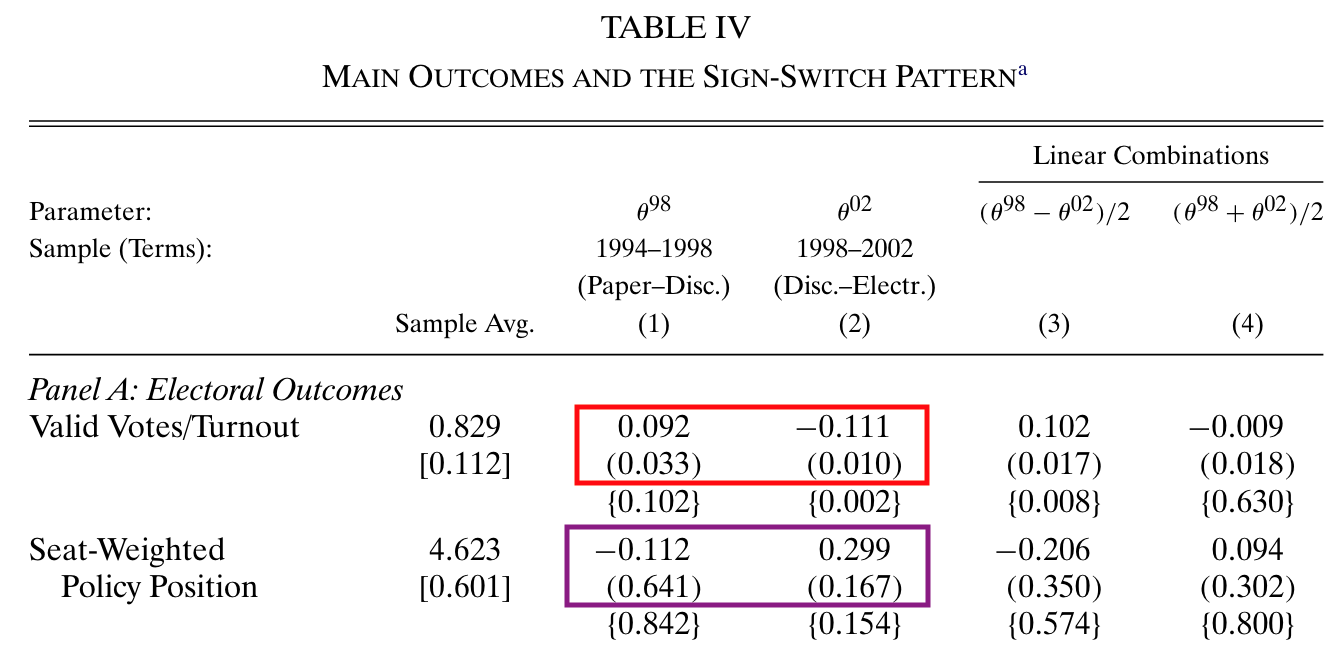
\includegraphics[width=0.8\textwidth]{inputs/fig7.png}
\end{figure}
\begin{itemize}
\pause \item $\theta_{98}$ is an estimate of the impact of EV on outcome $y_{i98}$
\pause \item Think of the dependent variable as the share of voters that EV affected in a state
\pause \item Sign-switch is interpreted as evidence of the effect of EV
\end{itemize}
\end{frame}
%---------------------------------------------------------------------

%---------------------------------------------------------------------
\begin{frame}{Political Participation and Policy}
\begin{figure}
\centering
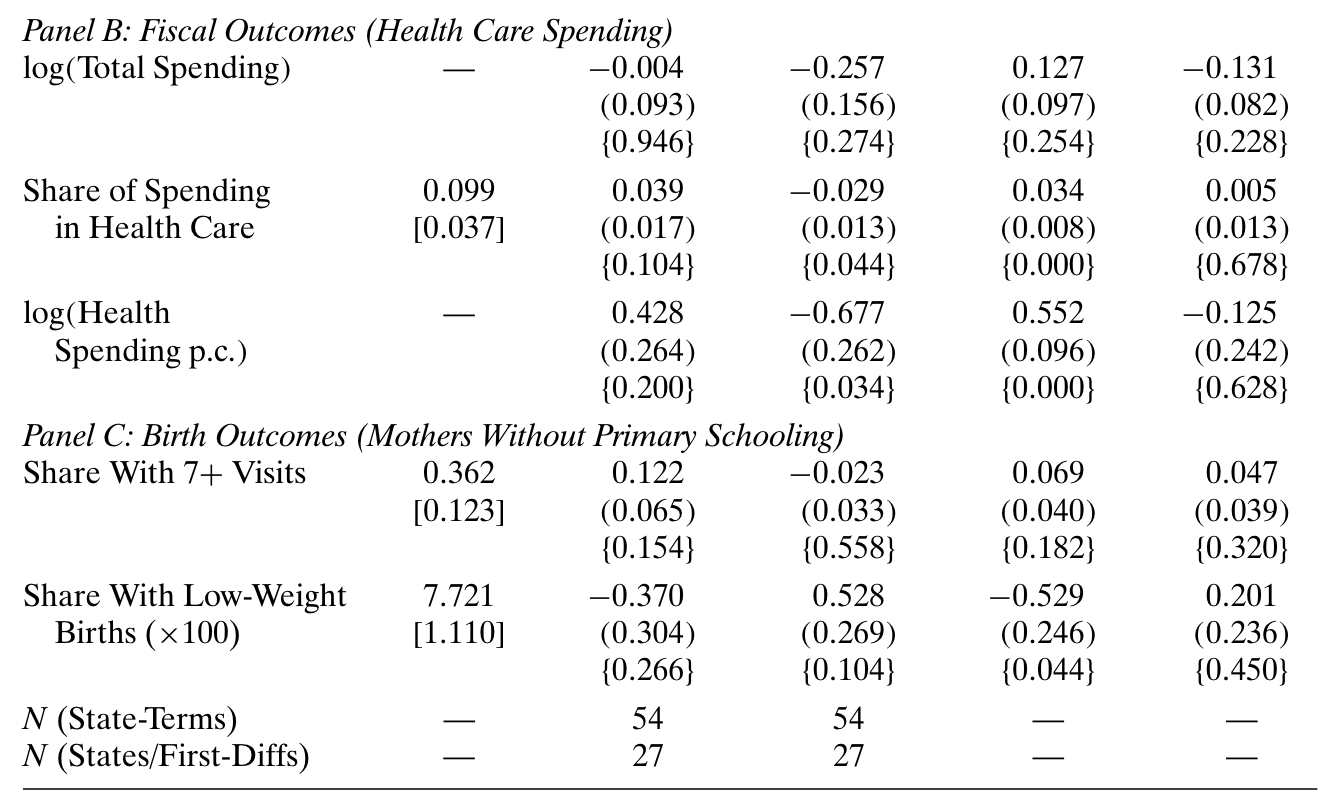
\includegraphics[width=0.6\textwidth]{inputs/fig8.png}
\end{figure}
\begin{itemize}
\pause \item Total spending seems unchanged
\pause \item But share of spending increases 
\pause \item Increased prenatal visits, birth weight
\end{itemize}
\end{frame}
%---------------------------------------------------------------------

%---------------------------------------------------------------------
\begin{frame}{Conclusion}
\begin{itemize}
\item This paper estimates the effects of EV 
\pause \item Promoted de facto enfranchisement of mainly less educated voters
\pause \item Increased spending in a sector particularly beneficial for the poor
\pause \item Also increased utilisation and health outcomes 
\pause \item So enfranchisement of poor voters matters for policy 
\pause \item Enables democracy to work as intended
\end{itemize}
\end{frame}
%---------------------------------------------------------------------

\section*{\href{https://academic.oup.com/restud/article/92/1/339/7627149}{\textcolor{blue}{Gulzar and Khan (2025)}} \\[5mm] 
\textnormal{\small{Good Politicians: Experimental Evidence on Motivations for Political Candidacy and Government Performance}}}

%---------------------------------------------------------------------
\begin{frame}{This Paper}
\begin{itemize}
\item Typically, we think of the intensive margin of politicians - how to make elected ones more responsive to citizens' preferences
\pause \item But the extensive margin is usually ignored
\pause \item How can we motivate good politicians to enter politics? 
\pause \item This paper asks: can portraying political office as enabling prosocial behaviour encourage good politicians? 
\pause \item In theory, it's ambiguous:
\begin{itemize}
    \pause \item Could encourage prosocial individuals to run
    \pause \item But may give selfish politicians a cover to run
    \pause \item And may crowd out competent, but personally-driven individuals
\end{itemize}
\end{itemize}
\end{frame}
%---------------------------------------------------------------------

%---------------------------------------------------------------------
\begin{frame}{Setting}
\begin{itemize}
\item Setting: Pakistan's 2015 local government reform 
\item Local level political entry decisions which could help understand the composition of the political class 
\item Village council elections - party affiliations not allowed
\item So centralised parties could not play a role in candidate selection
\end{itemize}
\end{frame}
%---------------------------------------------------------------------

%---------------------------------------------------------------------
\begin{frame}{The Experiment}
\begin{itemize}
\item 192 randomly selected villages, 9,310 people randomly selected 
\item Enumerators had private meetings and public meetings 
\item Treatments:
\begin{itemize}
    \item Neutral Script 
    \item Social Benefits Script
    \item Personal Benefits Script
\end{itemize}
\end{itemize}
\end{frame}
%---------------------------------------------------------------------

%---------------------------------------------------------------------
\begin{frame}{Meetings}
\begin{figure}
\centering
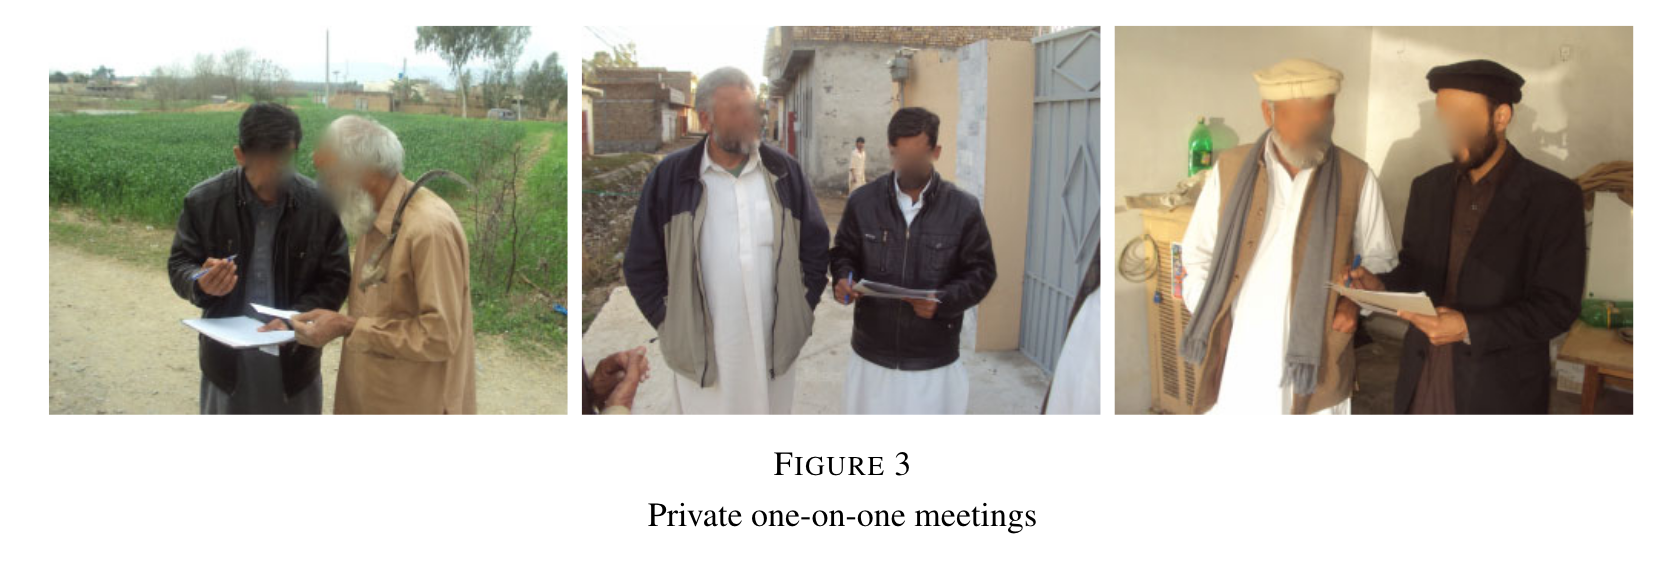
\includegraphics[width=0.7\textwidth]{inputs/fig9.png}
\end{figure}
\begin{figure}
\centering
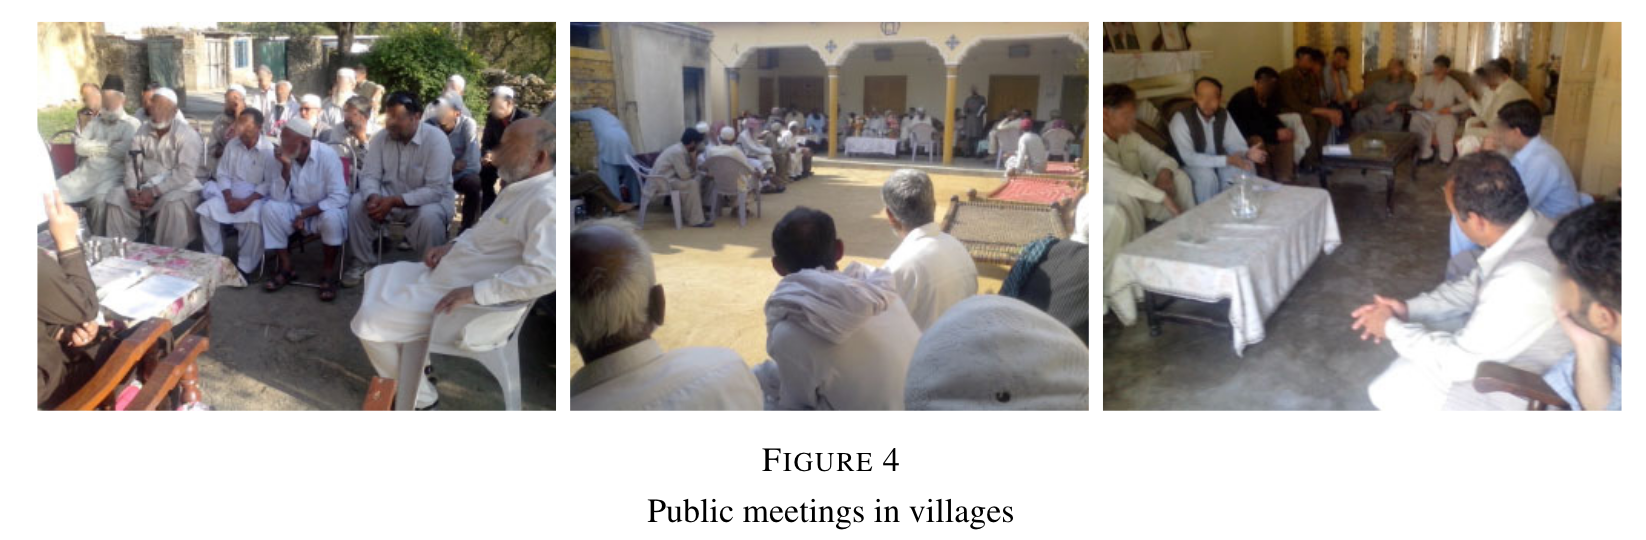
\includegraphics[width=0.7\textwidth]{inputs/fig10.png}
\end{figure}
\end{frame}
%---------------------------------------------------------------------

%---------------------------------------------------------------------
\begin{frame}{The Scripts}
\begin{itemize}
\item Neutral Script: ``You may be aware that for the first time elections on May 30th will elect a 10–15 member council at the village level. People above the age of 21 can contest these elections. There is not even an education requirement to contest. All you have to do is collect papers from the district office of the Election Commission, and submit them along with two references.''
\end{itemize}
\end{frame}
%---------------------------------------------------------------------

%---------------------------------------------------------------------
\begin{frame}{The Scripts}
    \begin{itemize}
    \item Social Benefits Script: Neutral Script and ``People who are elected to the village election will be given an excellent opportunity to do their part for the development of their area. Members of the village council will play an important role in improving the quality of government services in the village. They will work towards securing the welfare and rights of the poor. Working together with the district governments, they will improve village school and health facilities. An elected councillor will have a unique opportunity to address the problems of his neighbourhood, and this will make him the standard-bearer of social development for the village''
    \end{itemize}
    \end{frame}
    %---------------------------------------------------------------------

    %---------------------------------------------------------------------
\begin{frame}{The Scripts}
    \begin{itemize}
    \item Personal Benefits Script: Neutral Script and ``People who are elected to the village election will be given a excellent opportunity to move forward in politics, and gain respect and influence in the area. Members of the village council will be able to build connections with tehsil and district level politicians, which will open avenues for advancing in politics. Besides this, council members will also be able to enhance their influence in the village. They will be known as leaders in their neighbourhoods, and this get them more recognition. Their children will be able to build a network in the area, which will make their entry into politics easier.''
    \end{itemize}
    \end{frame}
    %---------------------------------------------------------------------
%---------------------------------------------------------------------
\begin{frame}{Design}
\begin{figure}
\centering
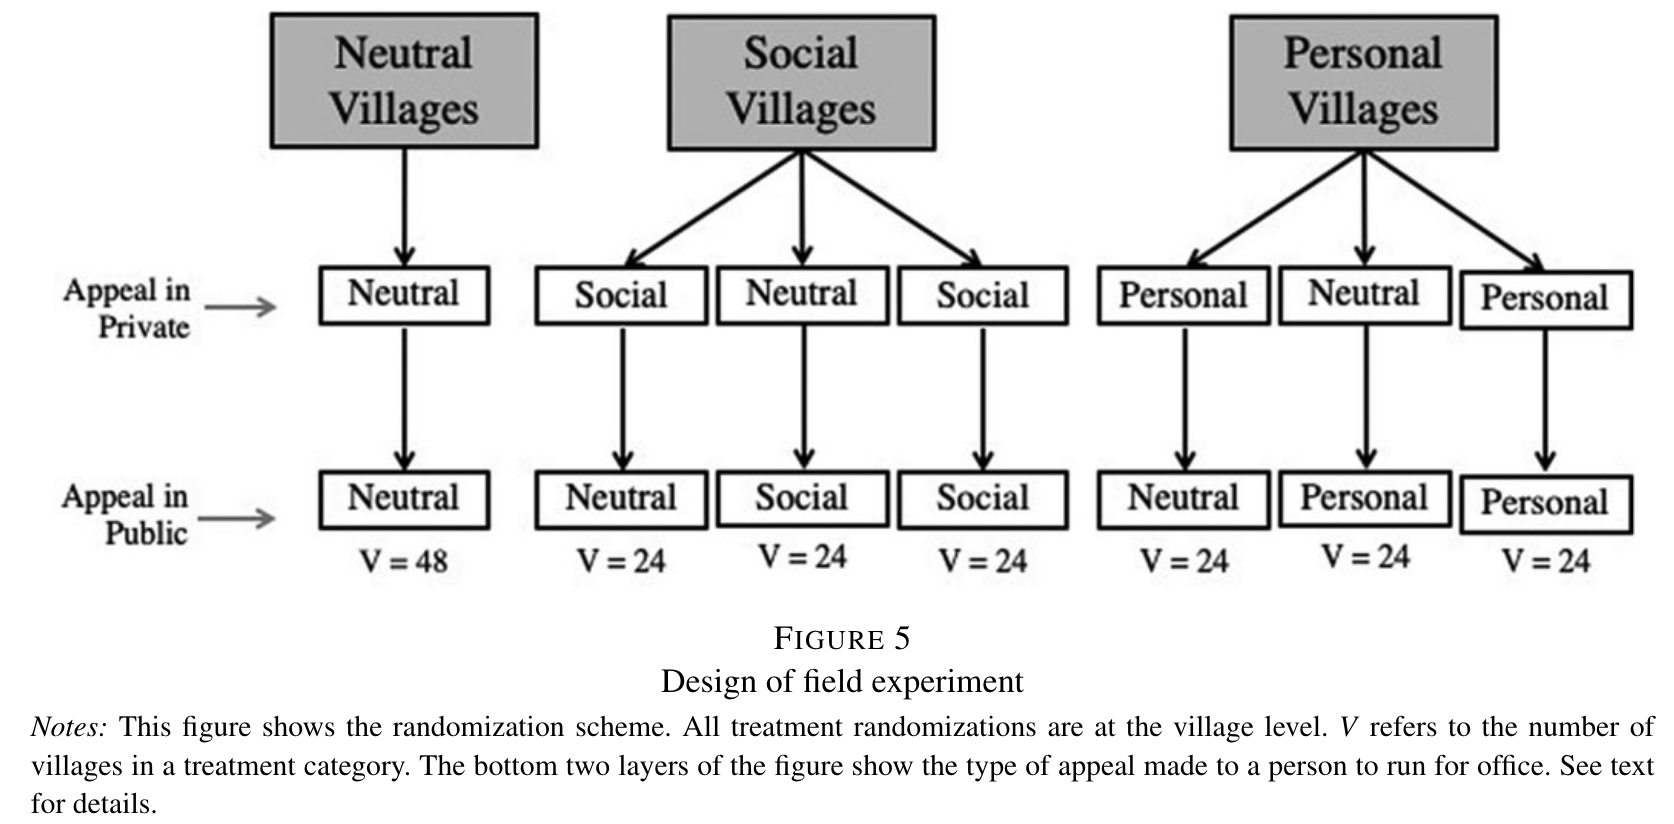
\includegraphics[width=1\textwidth]{inputs/fig11.png}
\end{figure}
\end{frame}
%---------------------------------------------------------------------

%---------------------------------------------------------------------
\begin{frame}{Political Entry Decisions}
    \begin{figure}
        \centering
        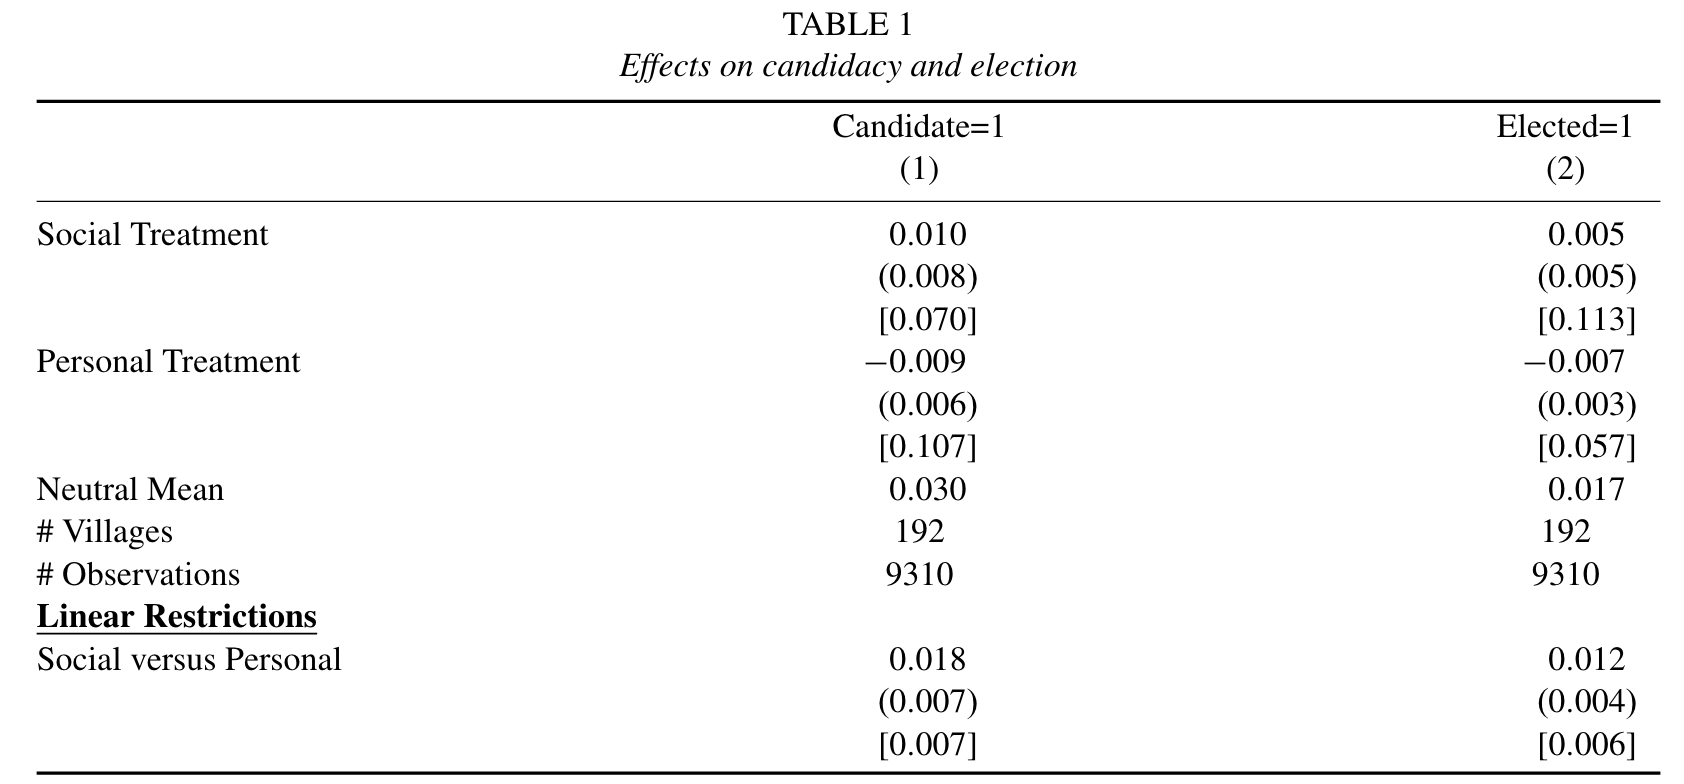
\includegraphics[width=0.7\textwidth]{inputs/table1.png}
        \end{figure}
\begin{itemize}
\item Relative to personal benefits, social benefits increase the probability of candidacy by 1.8 pp
\item An increase of 86\% 
\item Opposite effects for personal benefits relative to neutral treatment
\end{itemize}
\end{frame}
%---------------------------------------------------------------------

%---------------------------------------------------------------------
\begin{frame}{Do voters care to elect these new politicians?}
    \begin{figure}
        \centering
        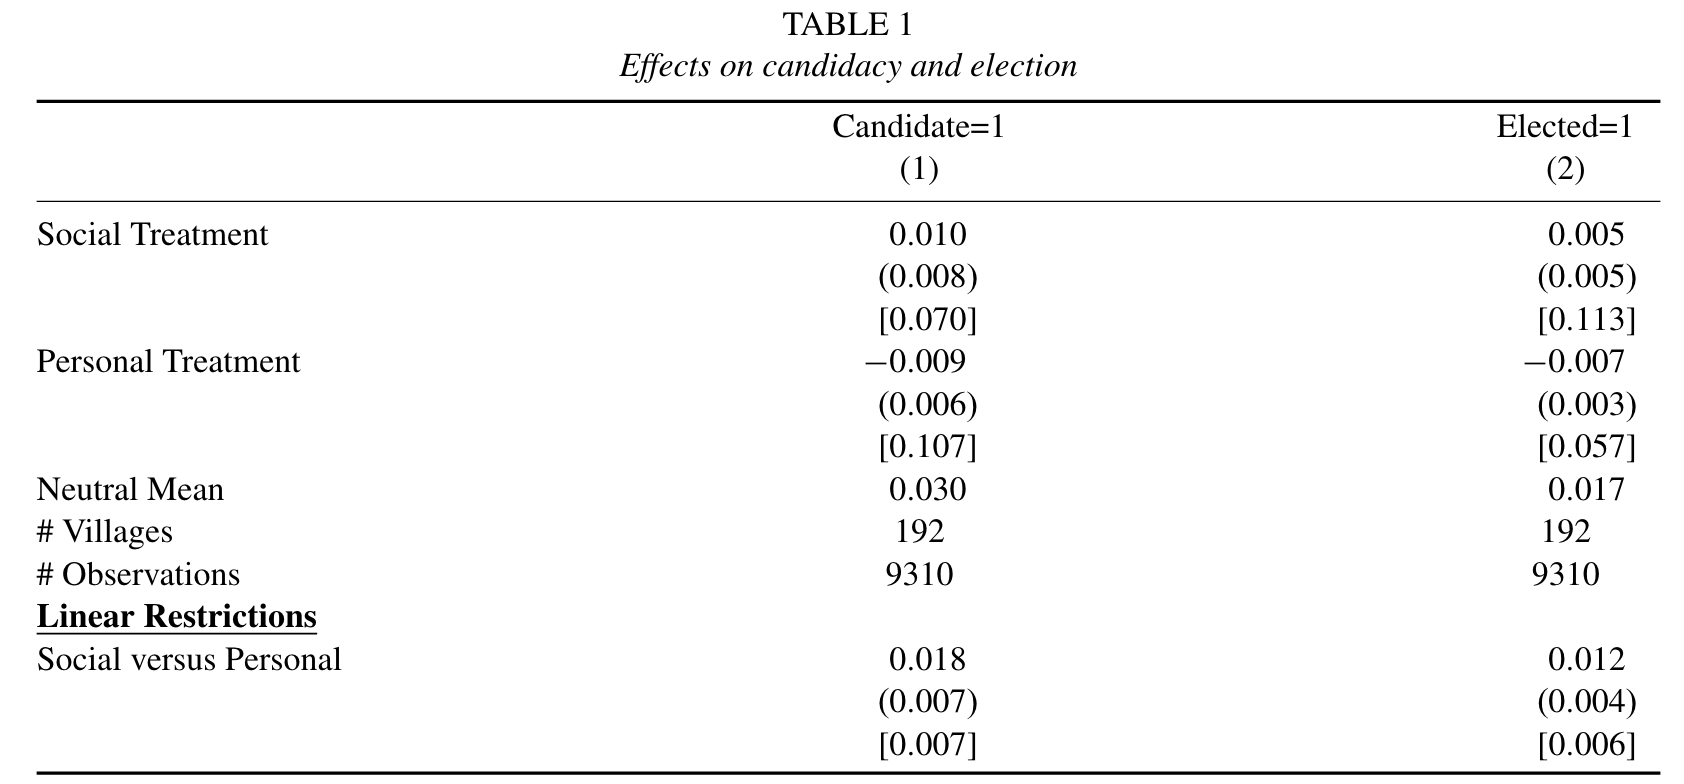
\includegraphics[width=0.8\textwidth]{inputs/table1.png}
        \end{figure}
        \begin{itemize}
    \item Probability of people getting elected to office is 1.2 pp higher when social benefits are emphasised
\end{itemize}
\end{frame}
%---------------------------------------------------------------------

%---------------------------------------------------------------------
\begin{frame}{Do these ``good'' politicians actually perform better?}
    \begin{figure}
        \centering
        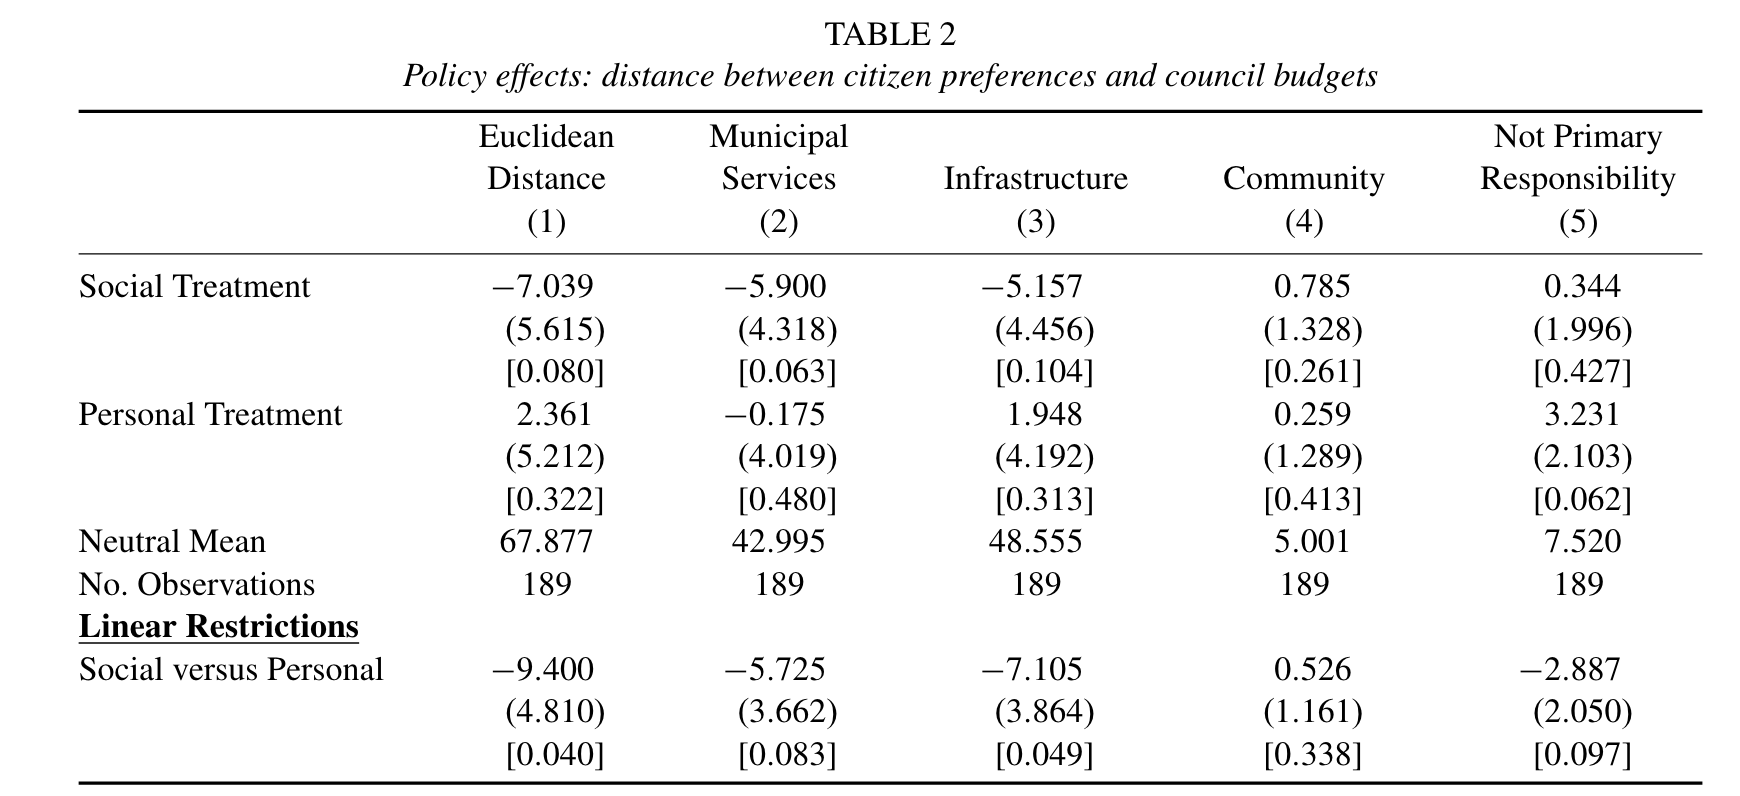
\includegraphics[width=0.8\textwidth]{inputs/table2.png}
        \end{figure}
\begin{itemize}
\item Elected councils in villages with social message spend their budgets in a manner that's more aligned with citizen preferences
\end{itemize}
\end{frame}
%---------------------------------------------------------------------

%---------------------------------------------------------------------
\begin{frame}{Conclusion}
\begin{itemize}
\item This paper presents new evidence on an important channel of improving representative democracy: the \textit{supply} of politicians
\item Non-monetary prosocial incentives can be particularly powerful in mobilising a political class that delivers more responsive policy to the electorate
\item When political office is presented as a means to serve the community, people who would not have otherwise run for office are more likely to do so
\item Prosocial encouragements at the candidacy stage also result is better alignment of downstream policy outcomes
\item Important policy implications: it is possible to improve the supply of politicians
\end{itemize}
\end{frame}
%---------------------------------------------------------------------

\section*{\href{https://www.lse.ac.uk/economics/Assets/Documents/personal-pages/robin-burgess/the-brazilian-amazons-double-reversal-of-fortune-manuscript.pdf}{\textcolor{blue}{Burgess et al. (2019)}} \\[5mm] 
\textnormal{\small{The Brazilian Amazon’s Double Reversal of Fortune}}}

%---------------------------------------------------------------------
\begin{frame}{Motivation}
\begin{itemize}
\item Environmental damage entails an externality - a market failure 
\item Requires government involvement to regulate or tax activity to correct this externality
\item State capacity to effectively regulate is weak in many developing countries
\item Political economy can be important 
\end{itemize}
\end{frame}
%---------------------------------------------------------------------

%---------------------------------------------------------------------
\begin{frame}{This Paper}
\begin{itemize}
\item Explore how national policies can exert regulatory control over conservation 
\item Exploit what happens at international borders 
\item One of the most important global ecosystems: the Amazon rainforest
\begin{itemize}
    \item The rate of deforestation will affect global warming
    \item The Amazon is a global public good
\end{itemize}
\end{itemize}
\end{frame}
%---------------------------------------------------------------------

%---------------------------------------------------------------------
\begin{frame}{Strategy}
\begin{itemize}
\item Satellite data on deforestation - even across borers, from 2000 - 2018 
\begin{itemize}
\item High resolution - can zoom in for precise effects 
\end{itemize}
\item In 2006, Brazil introduced deforestation policies
\item Spatial RDD design - popular strategy using borders for policy effects
\end{itemize}
\end{frame}
%---------------------------------------------------------------------

%---------------------------------------------------------------------
\begin{frame}{Satellite Data}
\begin{figure}
\centering
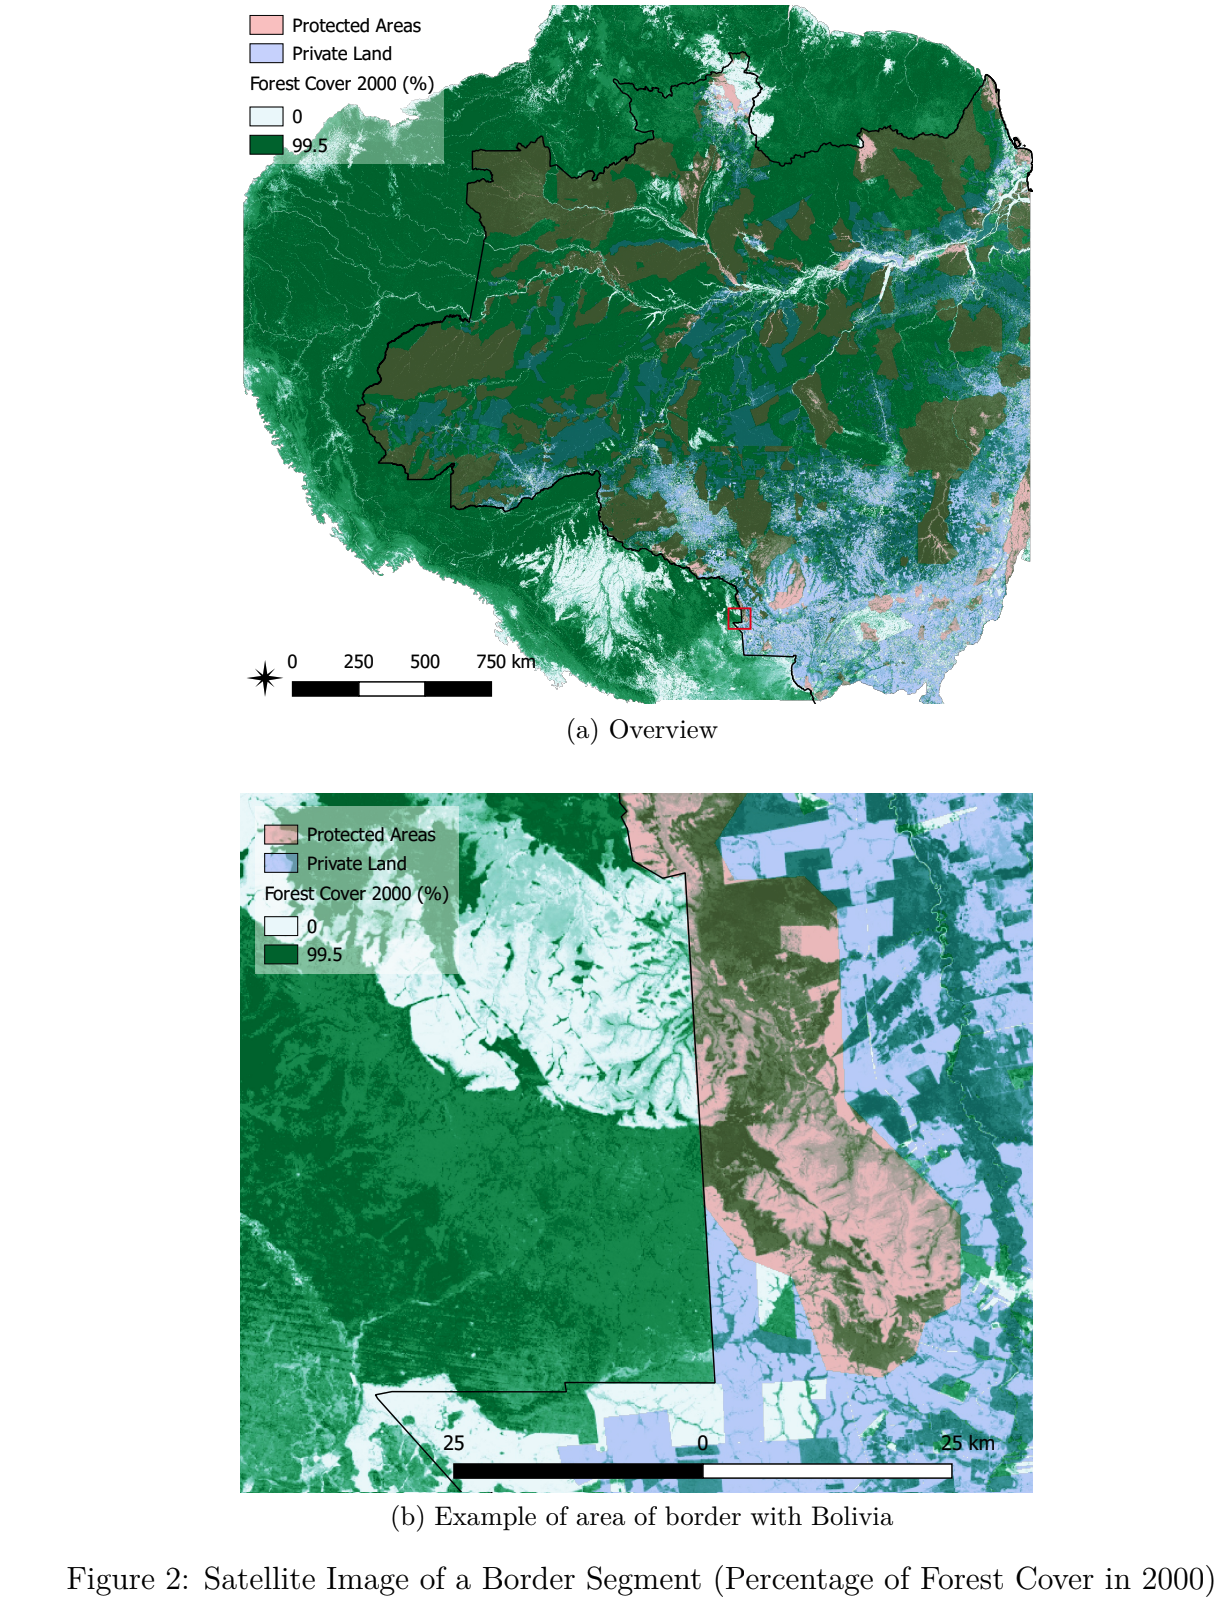
\includegraphics[width=0.4\textwidth]{../TA9/inputs/fig2.2.png}
\end{figure}
\end{frame}
%---------------------------------------------------------------------

%---------------------------------------------------------------------
\begin{frame}{Fact 1}
\begin{figure}
\centering
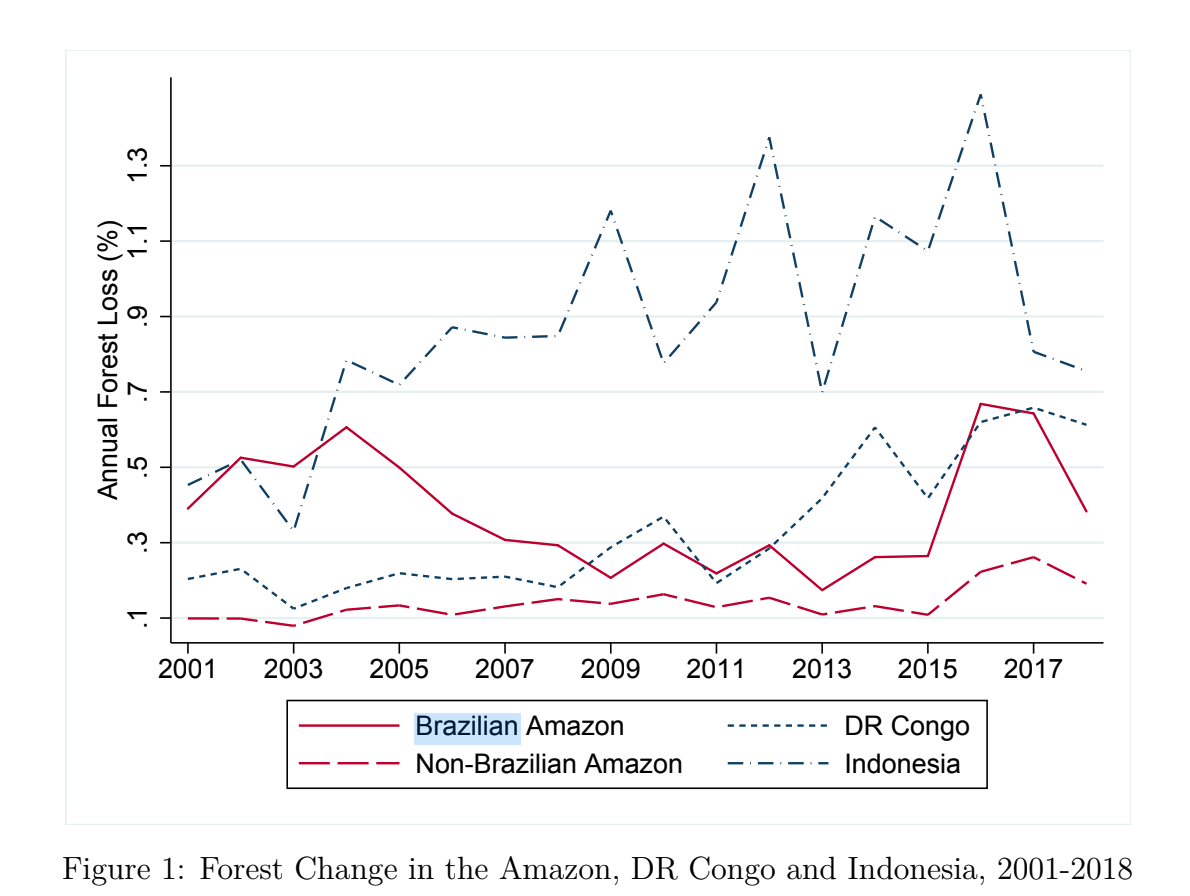
\includegraphics[width=0.6\textwidth]{../TA9/inputs/fig2.1.png}
\end{figure}
\begin{itemize}
\item Until 2005, deforestation level and rate significantly higher on the Brazilian side 
\end{itemize}
\end{frame}
%---------------------------------------------------------------------

%---------------------------------------------------------------------
\begin{frame}{Fact 1}
\begin{figure}
\centering
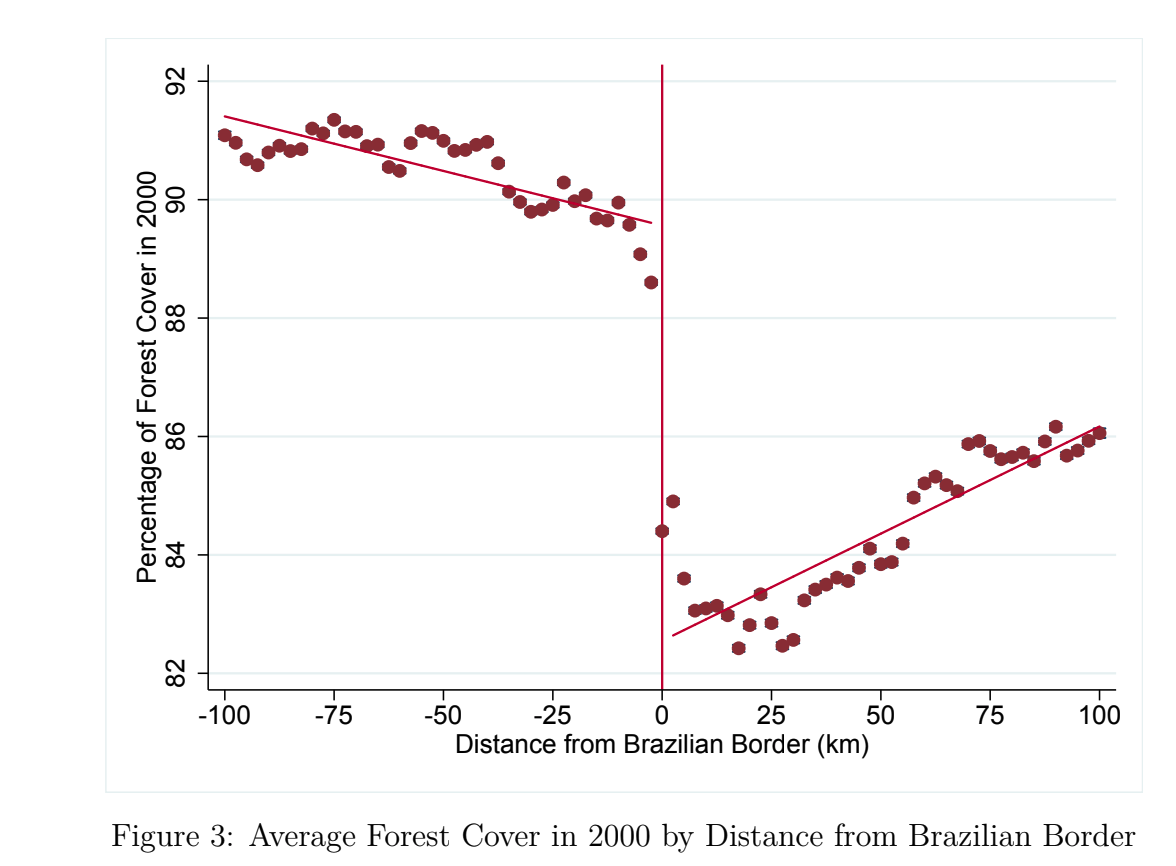
\includegraphics[width=0.56\textwidth]{../TA9/inputs/fig2.3.png}
\end{figure}
\begin{itemize}
\item Deforestation is visually apparent: forest cover drops sharply exactly at the national border.
\end{itemize}
\end{frame}
%---------------------------------------------------------------------


%---------------------------------------------------------------------
\begin{frame}{Fact 2}
\begin{figure}
\centering
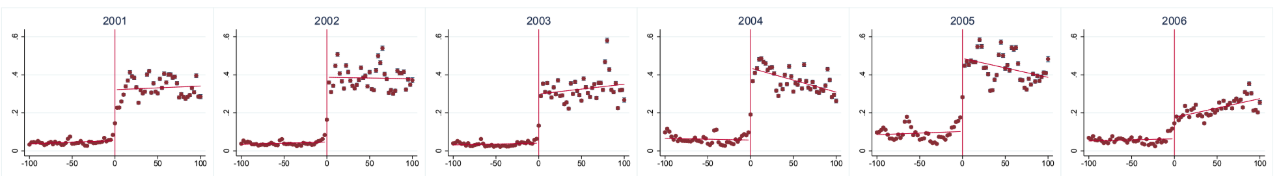
\includegraphics[width=1\textwidth]{../TA9/inputs/fig_2006.png}
\end{figure}
\begin{itemize}
\item Discontinuity in deforestation rates disappears in 2006 - the first reversal 
\end{itemize}
\end{frame}
%---------------------------------------------------------------------

%---------------------------------------------------------------------
\begin{frame}{What happened in 2006?}
\begin{itemize}
\item In 2003, in the Lula government, Marina Silva appointed as Minister of Environment
\item She was from the Amazon, and had a strong environmentalist stance
\item Law that allowed satellite-based deforestation detection system (DETER) to become a key tool
\item Sent in federal police and troops to arrest illegal loggers and confiscate their machinery
\end{itemize}
\end{frame}
%---------------------------------------------------------------------

%---------------------------------------------------------------------
\begin{frame}{Fact 3}
\begin{figure}
\centering
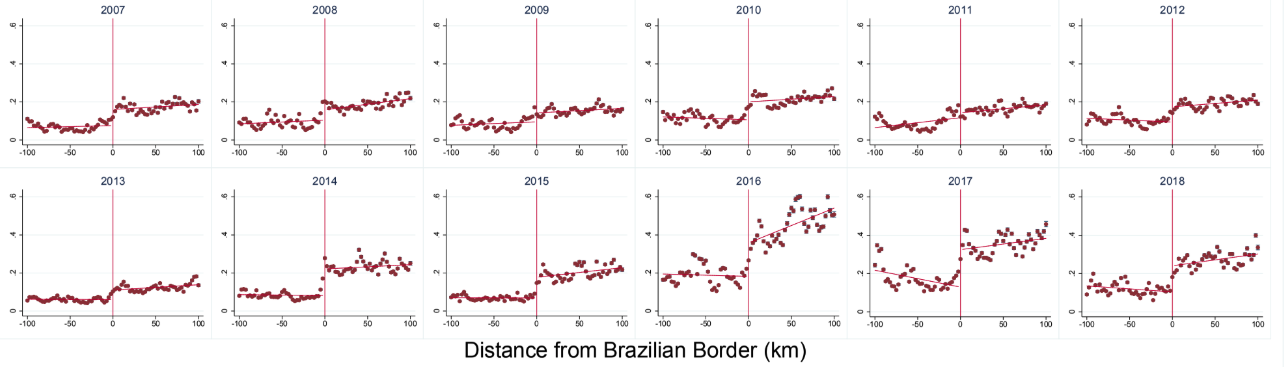
\includegraphics[width=1\textwidth]{../TA9/inputs/fig_post.png}
\end{figure}
\begin{itemize}
\item Positive effects relatively short-lived 
\item Deforestation resumes growing in 2014 - the second reversal
\end{itemize}
\end{frame}
%---------------------------------------------------------------------

%---------------------------------------------------------------------
\begin{frame}{What changed?}
\begin{itemize}
\item New government - gave amnesty to those engaged in illegal deforestation before 2008
\item 2014 was a politically turbulent year
\item Next president introduced laws that made it incentive-compatible for public land grabs
\end{itemize}
\end{frame}
%---------------------------------------------------------------------

%---------------------------------------------------------------------
\begin{frame}{The Double Reversal}
\begin{figure}
\centering
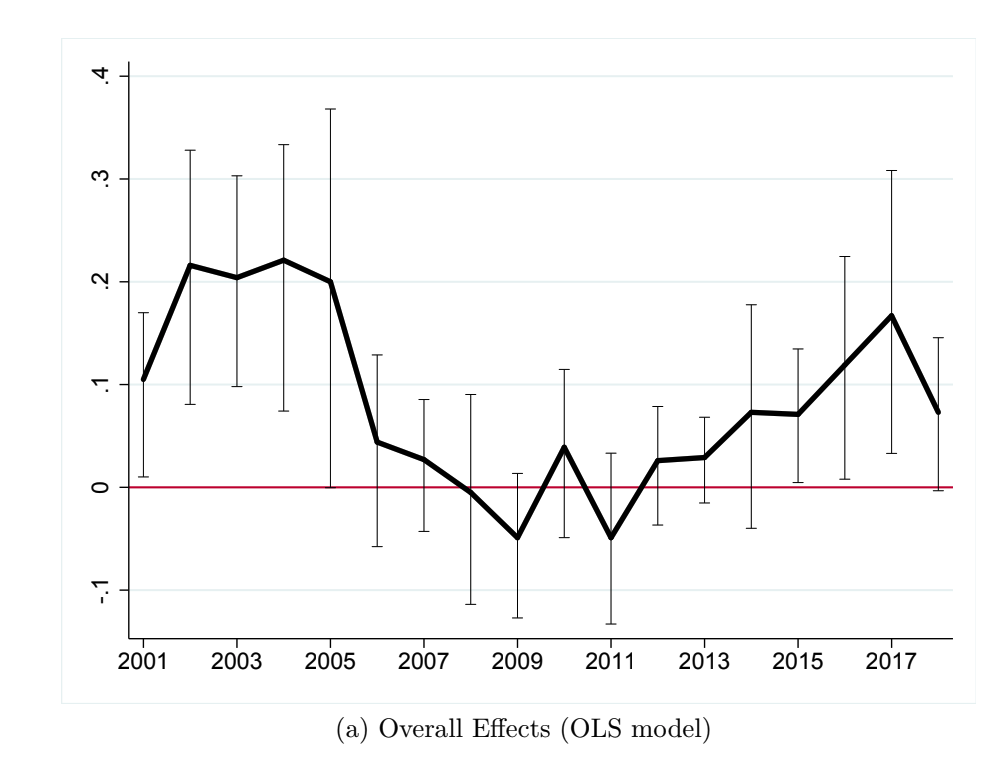
\includegraphics[width=0.6\textwidth]{../TA9/inputs/reversal.png}
\end{figure}
\end{frame}
%---------------------------------------------------------------------

%---------------------------------------------------------------------
\begin{frame}{Fact 4}
\begin{figure}
\centering
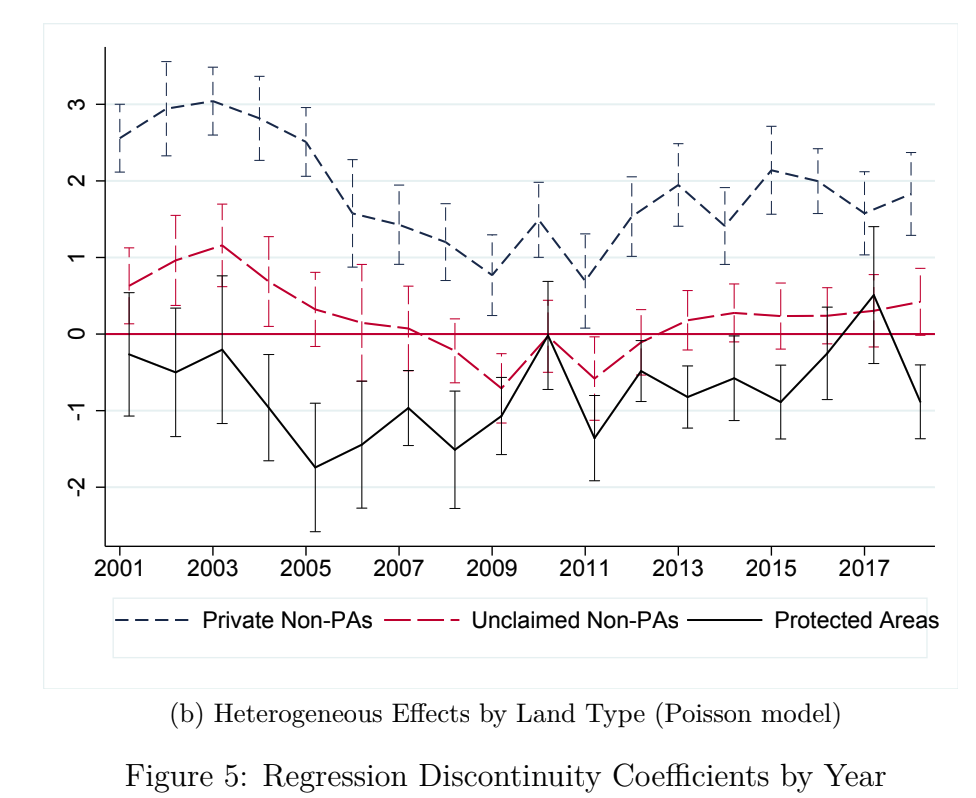
\includegraphics[width=0.5\textwidth]{../TA9/inputs/fig_land_use.png}
\end{figure}
\begin{itemize}
\item Land use restrictions matter 
\item Protected areas have always been less deforested
\end{itemize}
\end{frame}
%---------------------------------------------------------------------

%---------------------------------------------------------------------
\begin{frame}{Conclusion}
\begin{itemize}
\item Combined, these results demonstrate the reach of the Brazilian state to exploit or conserve its natural resources
\item Suggest that rapid deforestation in early 2000s was a consequence of a pro-exploitation policy environment 
\item Policy stance rapidly reversed in 2006-2013 with laws introduced 
\item But the position stalled and reversed in the post-2013 period with economic and political crisis collided with weakened forest conservation laws 
\item So state capacity does matter!
\end{itemize}
\end{frame}
%---------------------------------------------------------------------

\section*{The Curse of Natural Resources}

%---------------------------------------------------------------------
\begin{frame}{What is it?}

\begin{itemize}
\item The observation that countries rich in natural resources tend to perform badly
\item Also called the paradox of plenty or the resource curse
\item Sachs and Warner maybe the first to document this using econometrics in a paper in 1995
\end{itemize}
\end{frame}
%---------------------------------------------------------------------

%---------------------------------------------------------------------
\begin{frame}{Descriptive Evidence}
\begin{figure}
\centering
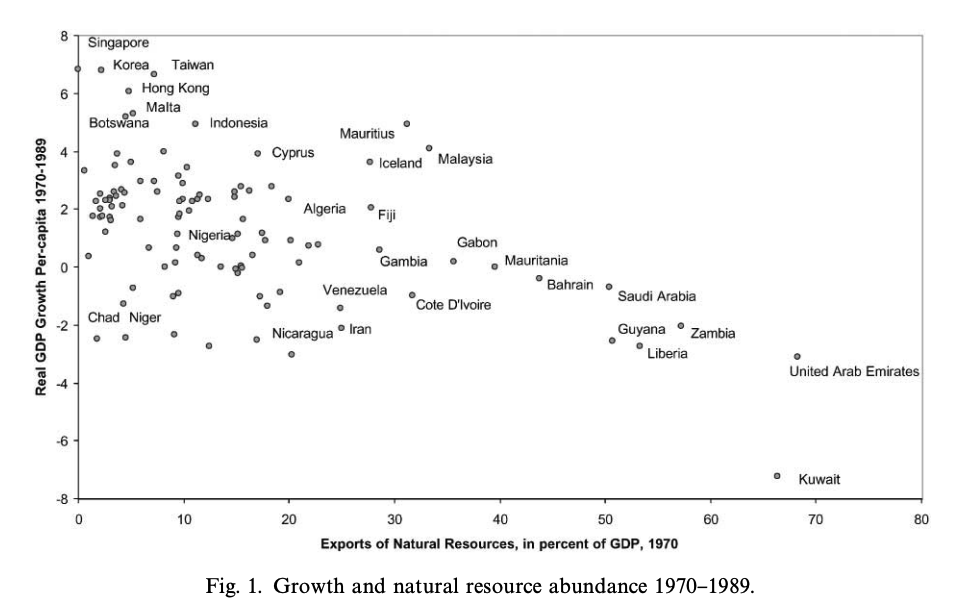
\includegraphics[width=0.6\textwidth]{../TA9/inputs/fig1.png}
\end{figure}
\begin{itemize}
\item No countries with extremely abundant natural resources in 1970 grew rapidly for the next 20 years
\end{itemize}
\end{frame}
%---------------------------------------------------------------------

%---------------------------------------------------------------------
\begin{frame}{Descriptive Evidence - Persistence}
\begin{figure}
\centering
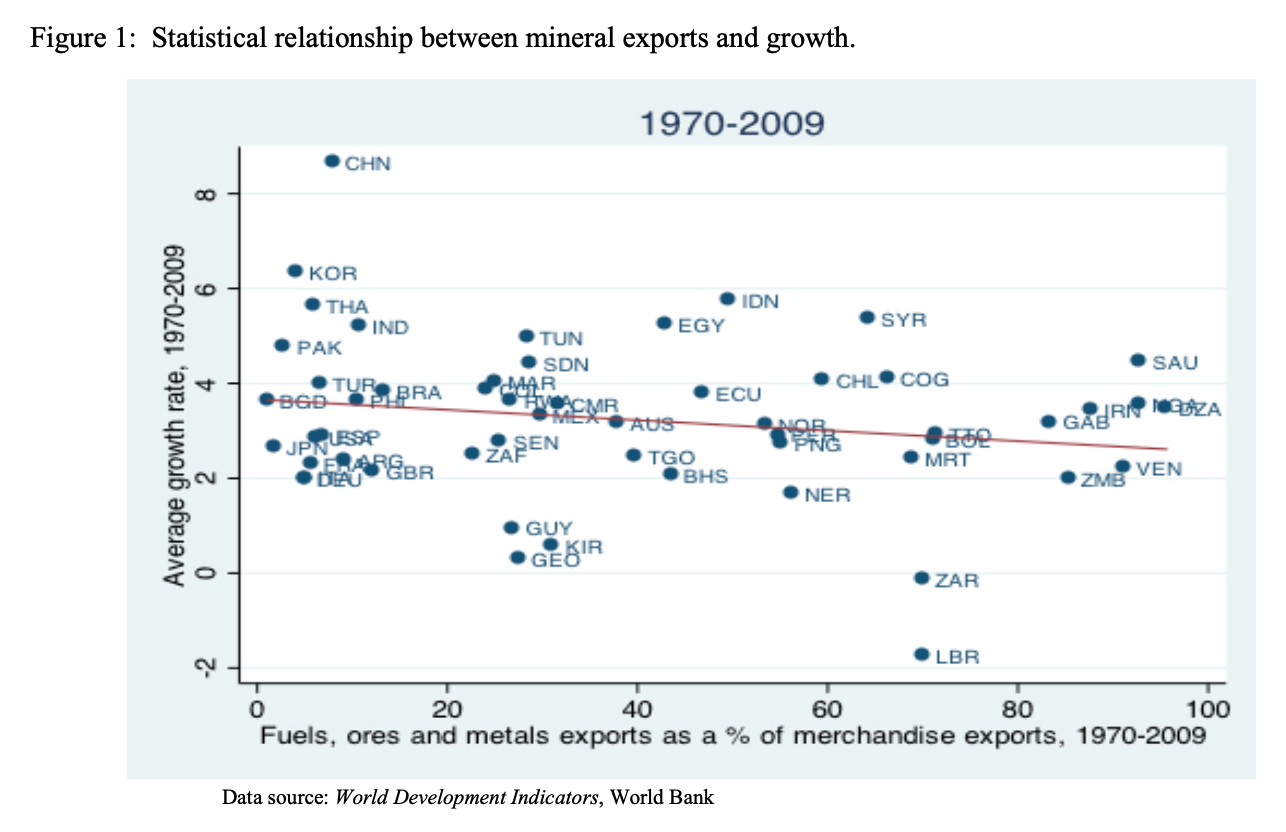
\includegraphics[width=0.55\textwidth]{../TA9/inputs/fig2.png}
\end{figure}
\begin{itemize}
\item Conspicuously high growth and low natural resources are China, Korea
\pause \item Conspicuously high resources and low growth are Gabon, Venezuela and Zambia. 
\pause \item Not very strong negative relationship...
\pause \item But clearly no positive relationship
\end{itemize}
\end{frame}
%---------------------------------------------------------------------


%---------------------------------------------------------------------
\begin{frame}{Possible Mechanisms I}

\begin{itemize}
\item Long run trend of world prices for commodities
\begin{itemize}
    \pause \item Could be downward
    \pause \item But could also be upward 
    \pause \item No convincing empirical evidence
\end{itemize}
\item Volatility in commodity prices 
\begin{itemize}
    \pause \item Commodity prices are highly volatile
    \pause \item Cyclical shifts of factors of production - transaction costs 
    \pause \item Low short-run elasticities - large price responses to small shocks
\end{itemize}
\end{itemize}
\end{frame}
%---------------------------------------------------------------------

%---------------------------------------------------------------------
\begin{frame}{Possible Mechanisms II}
\begin{itemize}
\item Permanent crowding out of manufacturing 
\begin{itemize}
    \pause \item How does it happen?
    \pause \item Positive wealth shocks $\rightarrow$ excess demand for non-traded goods $\rightarrow$ prices $\uparrow$ $\rightarrow$ manufacturing profits $\downarrow$ $\rightarrow$ manufacturing $\downarrow$ growth $\downarrow$
    \pause \item Diversification is desirable - in particular, industrial policy 
\end{itemize}
\end{itemize}
\end{frame}
%---------------------------------------------------------------------

%---------------------------------------------------------------------
\begin{frame}{Crowding out of manufacturing?}
\begin{figure}
\centering
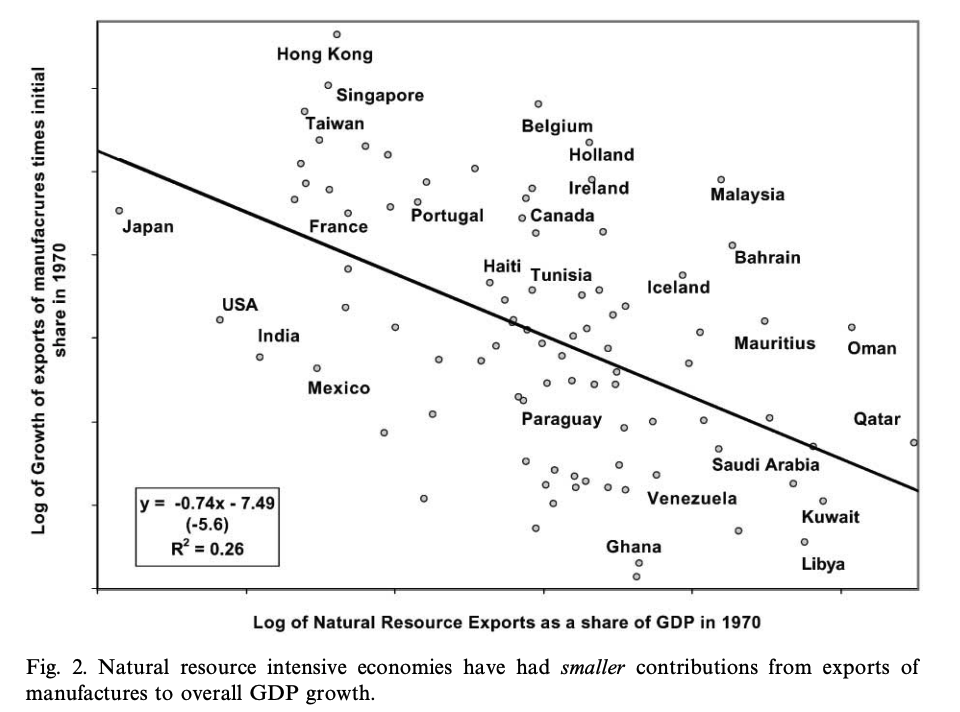
\includegraphics[width=0.5\textwidth]{../TA9/inputs/fig3.png}
\end{figure}
\begin{itemize}
\item Resource abundance tended to render the export sectors uncompetitive
\item So never successfully pursued export-led growth
\end{itemize}
\end{frame}
%---------------------------------------------------------------------

%---------------------------------------------------------------------
\begin{frame}{Possible Mechanisms III}
\begin{itemize}
\item Autocractic or oligarchic governance
\begin{itemize}
    \pause \item Elicits a political contest for resource rents
    \pause \item Extractive industries emerged 
    \pause \item Which commodities? Oil, minerals, cocoa, coffee, plantation crops
\end{itemize}
\item Anarchic institutions
\begin{itemize}
    \pause \item Unenforeceable property rights - tragedy of the commons
    \pause \item Unsustainably rapid depletion of resources - solution to privatise?
    \pause \item Civil war - factions fight for control of resources (Angola, Sudan) 
\end{itemize}
\pause \item Cyclical expansion of the non-traded sector via the Dutch Disease
\begin{itemize}
    \pause \item Currency appreciates $\rightarrow$ govt. spending $\uparrow$ $\rightarrow$ non-traded sector prices $\uparrow$ $\rightarrow$ shift of labour and land from traded to non-traded sector
    \pause \item Economy more vulnerable to resource-related shocks
\end{itemize}
\end{itemize}
\end{frame}
%---------------------------------------------------------------------

\end{document}
